\label{Chapter1}

\chapter{Introduction}

\section{Motivation}
A space exploration vehicle designed to move across the surface of a planet,
besides Earth, is called a planetary rover as of its ability to "rove over"
an unknown terrain.
Planetary rovers are used to collect valuable data and samples such as
pictures, dust and rocks, which are later analyzed by scientists to enrich
our understanding regarding the universe.

Past missions have sent robots to the Moon and Mars (Figure
\ref{fig:mars_sites}) with the NASA's Curiosity being the last rover to
land on Mars in 2011.
Future missions do not differ much, as new lunar rovers are about to launch
in the next years and Mars rovers are currently under development scheduled
to be sent to Mars in 2020.

Such missions utilize a great amount of time and effort to build,
launch and finally operate.
Our interest lies in the operation challenges that are caused by the fact
that no constant communication can be achieved.
As an example, commanding messages can take up to 21 minutes to travel
between the Earth and Mars and bandwidth limitations can limit the number
of messages that can be sent.
This compounded to the unpredictable and unsafe conditions of
an unknown terrain such as the Mars surface which is full of rocks,
could lead to destructive system crashes of a costly mission.

Thus, we emphasize the need of a real time platform that will provide the
capability of autonomous operation with low supervision from ground control
as far as navigation is concerned.

\begin{figure}[h!]
    \centering
    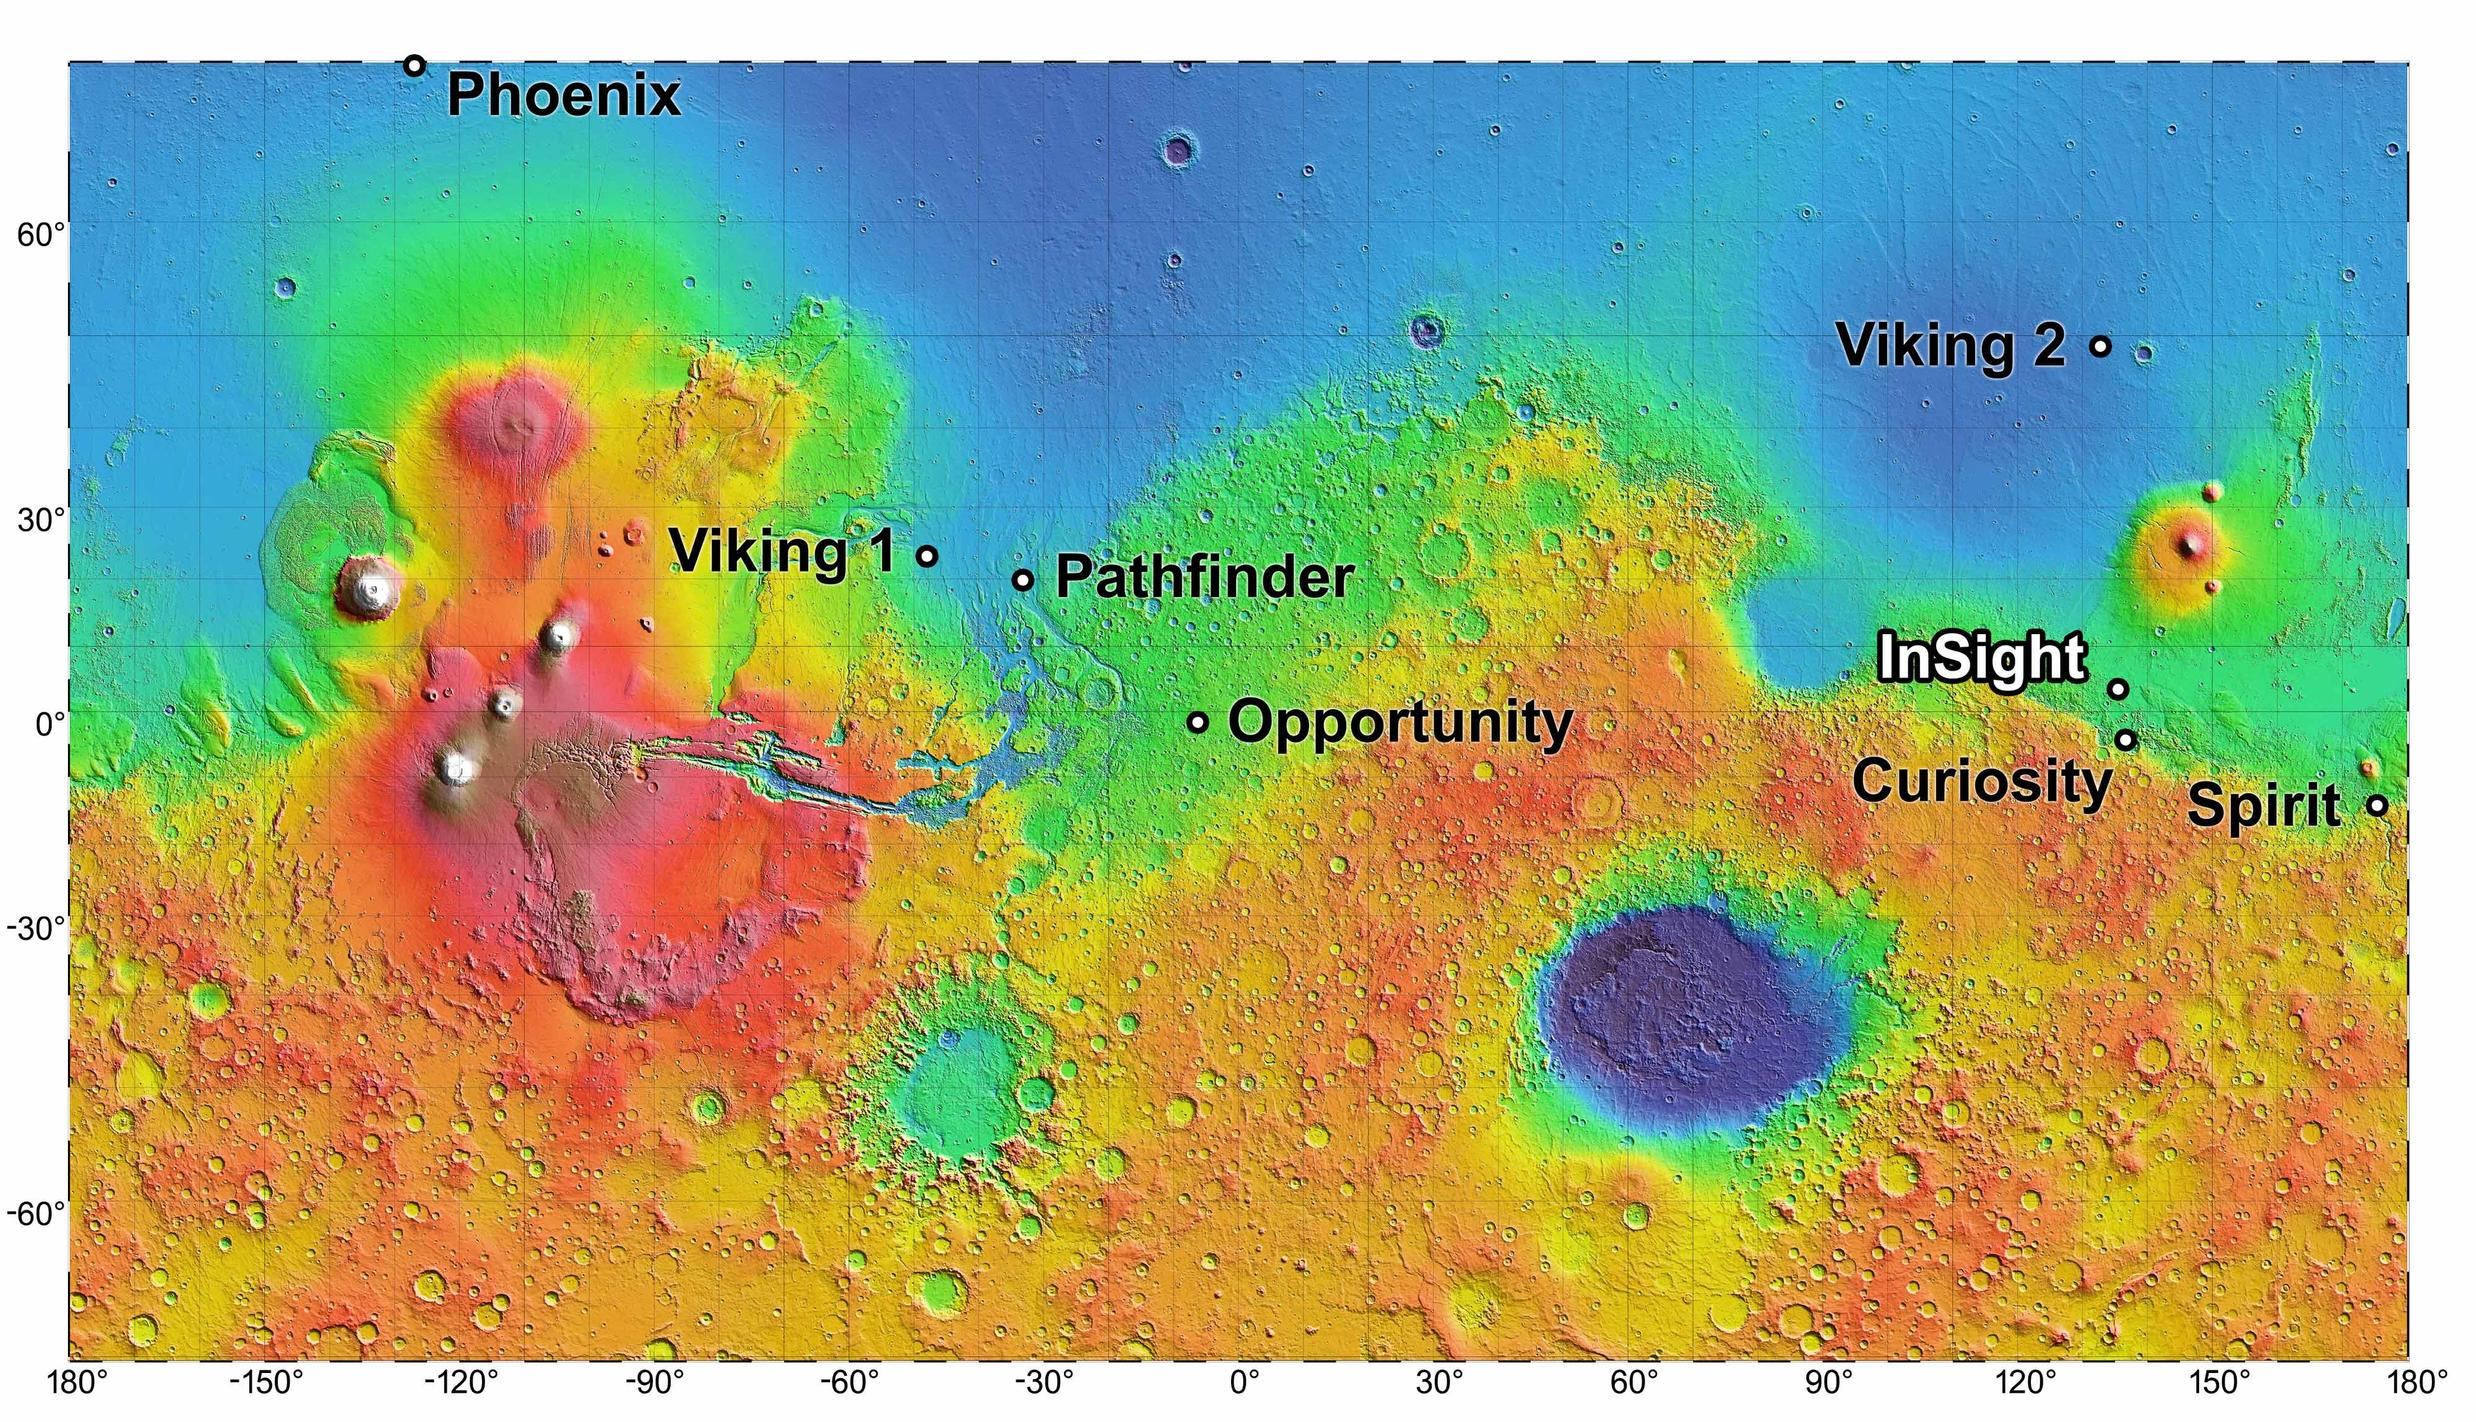
\includegraphics[scale=0.15]{mars_sites}
    \decoRule
    \caption[Mars landing sites]{
        Mars landing sites of rovers and landers from NASA's past missions.
    }
    \label{fig:mars_sites}
\end{figure}

\section{Problem Statement}

In order to navigate autonomously in extreme terrains, rovers need to
accurately perceive the 3D environment around them based on sensory
information.
Terrains that classify as extreme are areas with high variance in elevation
and great morphological anomalies, such as rocks and craters.

This thesis actively researches the challenges of perception in such terrains
in a planetary context and mainly focuses on two problems.
The first is the relative localization of the robot and the local mapping
of its surroundings in order to provide autonomous navigation capabilities
to it.
The second problem is the global localization of the robot, which is the
elimination of the accumulated drift from relative localization in long
range scenarios.

Specifically, given as inputs:
\begin{enumerate*}[label=(\roman*)]
    \item an initial prediction about the robot's movement,
    \item a detailed 3D representation of the close surroundings of the robot
        and
    \item an a priori low resolution map of the greater area,
\end{enumerate*}
the purpose is to output:
\begin{enumerate*}[label=(\roman*)]
    \item an accurate estimation of the position and orientation of the
        robot in a global reference frame and
    \item a local (robot-centric) map that represents the height of
        the environment.
\end{enumerate*}

\subsection{Presumptions}

In order to tackle the aspect of the problem that is of most interest,
we first assume the following:

\begin{itemize}
    \item a low resolution global map is available to the system at any time
    \item the initial global position of the robot is known
    \item the environment is static, i.e. is does not contain any
        moving objects
    \item the environment is unknown, i.e. there are no high resolution
        a priori maps available
    \item the terrain is single layered, i.e. there are no bridges or caves
\end{itemize}

\section{Literature Review}

\subsection{SLAM}

\begin{itemize}
    \item  What is SLAM
        \begin{itemize}
            \item typical explanation in literature
            \item categories
        \end{itemize}
    % TODO: Add typical math expressions
    \item How is SLAM implemented
        \begin{itemize}
            \item volumetric/feature based approaches
            \item grid-based fast slam
            \item etc. etc. etc.
        \end{itemize}
\end{itemize}

\subsection{Planetary Absolute Localization}

Mention how is absolute localization achieved in planetary applications

\begin{itemize}
    \item Feature based approaches
    \item Skyline based approaches
    \item map based approaches
\end{itemize}

\section{Thesis Objectives and Outline}

\subsection{Research Objectives}

The main objectives of this thesis in terms of research are:

\begin{itemize}
    \item to utilize SLAM techniques for the localization and mapping
        of a planetary rover
    \item to develop a novel technique for minimizing the localization
        drift with global map matching
    \item to determine under which circumstances (i.e. resolutions of
        local and global maps) can the orbital imagery be useful for
        solving the SLAM problem
    \item to examine and quantify the gains (i.e. high resolution map for
        navigation purposes and absolute localization) and loses
        (i.e. processing overhead) of such approach.
\end{itemize}

\subsection{Outline}

The remainder of this thesis is organized as follows:
\begin{itemize}
    \item \textbf{Chapter 2} introduces a detailed approach for solving the
        SLAM problem in a planetary context using global map matching,
    \item \textbf{Chapter 3} deals with the implementation details and
        the tools used to develop a working system overall,
    \item \textbf{Chapter 4} presents the results of the experiments that
        were carried out in order to validate the approach and
    \item \textbf{Chapter 5} concludes with a summary, thoughts about future
        directions as well as possible applications.
\end{itemize}

